245. \begin{figure}[ht!]
\center{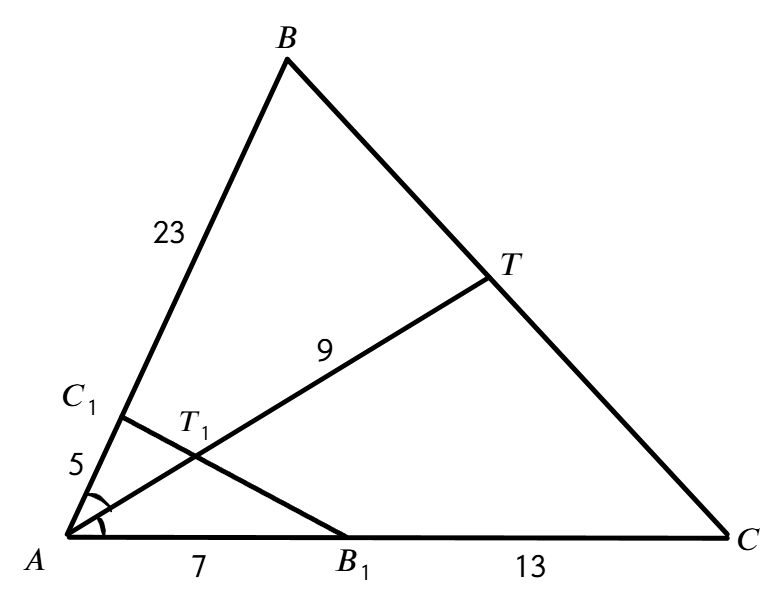
\includegraphics[scale=0.35]{g8-242.png}}
\end{figure}\\
Найдём $AB=AC_1+C_1B=5+23=28$ и $AC=AB_1+B_1C=7+13=20.$ Треугольники $ABC$ и $AB_1C_1$ подобны по первому признаку: $\cfrac{AB}{AB_1}=\cfrac{AC}{AC_1}=4,$ угол $A$ --- общий. Тогда с тем же коэффициентом подобия относятся друг к другу и их биссектрисы: $\cfrac{AT}{AT_1}=4,\ \cfrac{AT_1+9}{AT_1}=4,\ 3AT_1=9,\ AT_1=3.$\\
